\chapter{Software}

\begin{tikzpicture}[->,>=stealth']

	
	
	\node[state]	(q1)							 {$q_1$};
	\node[state,node distance=2cm]	(q0) [left of=q1]  {$q_0$};
	\node[state,node distance=2cm]	(q2) [right of=q1]  {$q_2$};
	\node[state,node distance=2cm]	(q3) [right of=q2]  {$q_3$};
	\node[initial,state,accepting,node distance=3cm]	(q4) [below of=q1]	{$q4$};
	
	\path[->]	(q4) edge [loop below] node[auto] {$a\lor \neg d$} (q4);
	\path[->]	(q4) edge [bend left=20] node[auto] {$\neg a \land d$} (q0);
	\path[->]	(q0) edge [bend left=20] node[auto] {$a$} (q4);
	\path[->]	(q0) edge [] node[auto] {$\neg a$} (q1);
	\path[->]	(q1) edge [] node[auto] {$a$} (q4);
	\path[->]	(q1) edge [] node[auto] {$\neg a$} (q2);
	\path[->]	(q2) edge [] node[auto] {$a$} (q4);
	\path[->]	(q2) edge [loop above] node[auto] {$\neg a \land \neg b$} (q2);
	\path[->]	(q2) edge [bend right=45] node[above] {$\neg a \land b$} (q0);
	\path[->]	(q2) edge [] node[above] {$c$} (q3);
	\path[->]	(q3) edge [bend left=20] node[auto] {$always$} (q4);
\end{tikzpicture}

\begin{itemize}
	\item \textbf{$a$:} reset = true
	\item \textbf{$b$:} Alle Pixel im aktuellen Kernel analysiert = true
	\item \textbf{$c$:} Alle Pixel des Bildes analysiert = true	
	\item	\textbf{$d$:} Beginn eines neuen Frames = true
\end{itemize}



\begin{itemize}
	\item \textbf{q\textsubscript{0}:} Erster Warte-Zustand zwischen dem Anlegen der Speicheradresse am Block RAM und dem Auslesen der Daten
	\item \textbf{q\textsubscript{1}:} Erster Warte-Zustand zwischen dem Anlegen der Speicheradresse am Block RAM und dem Auslesen der Daten
	\item \textbf{q\textsubscript{2}:} Analysieren der ausgelesenen Daten
	\item \textbf{q\textsubscript{3}:} Überschreiben der gefundenen ROIs von einem Buffer in das Ausgaberegister	
	\item \textbf{q\textsubscript{4}:} Reset-Zustand, der die Variablen auf einen Anfangszustand zurück setzt	
\end{itemize}

\textbf{Beschreibung der Pixel-Analyse:}\\
Durch das Anlegen einer Adresse an den Block-RAM, wird das Auslesen initialisiert und nach 2 Clock-Takten können die Daten der entsprechenden Adresse, am Ausgang des Speichers,  abgegriffen werden.
Pro Speichereinheit enthält der RAM 255 Bit Daten, die sich aus 32 Pixeln mit je 8 Bit Intensitätswert, zusammensetzen. Für diesen Vorgang sind die Zustände $q0$ und $q1$ zuständig.\\
Die Analyse wird pixelweise durchgeführt. Überschreitet die Intensität des Pixels einen definierten Grenzwert, wird er als Kandidat für einen Spot in Betracht gezogen. Im Anschluss wird überprüft, ob der Pixel bereits in einer ROI enthalten ist, sollte dies nicht der Fall sein, werden basierend auf den Parametern ROI\_width und ROI\_height, 2 Punkte ermittelt, die ein Rechteck um den Spot aufspannen. Die beiden Punkte entsprechen der linken oberen und der rechten unteren Ecke des Rechteckes und werden entsprechend angepasst, damit sie definitiv im Bild liegen.

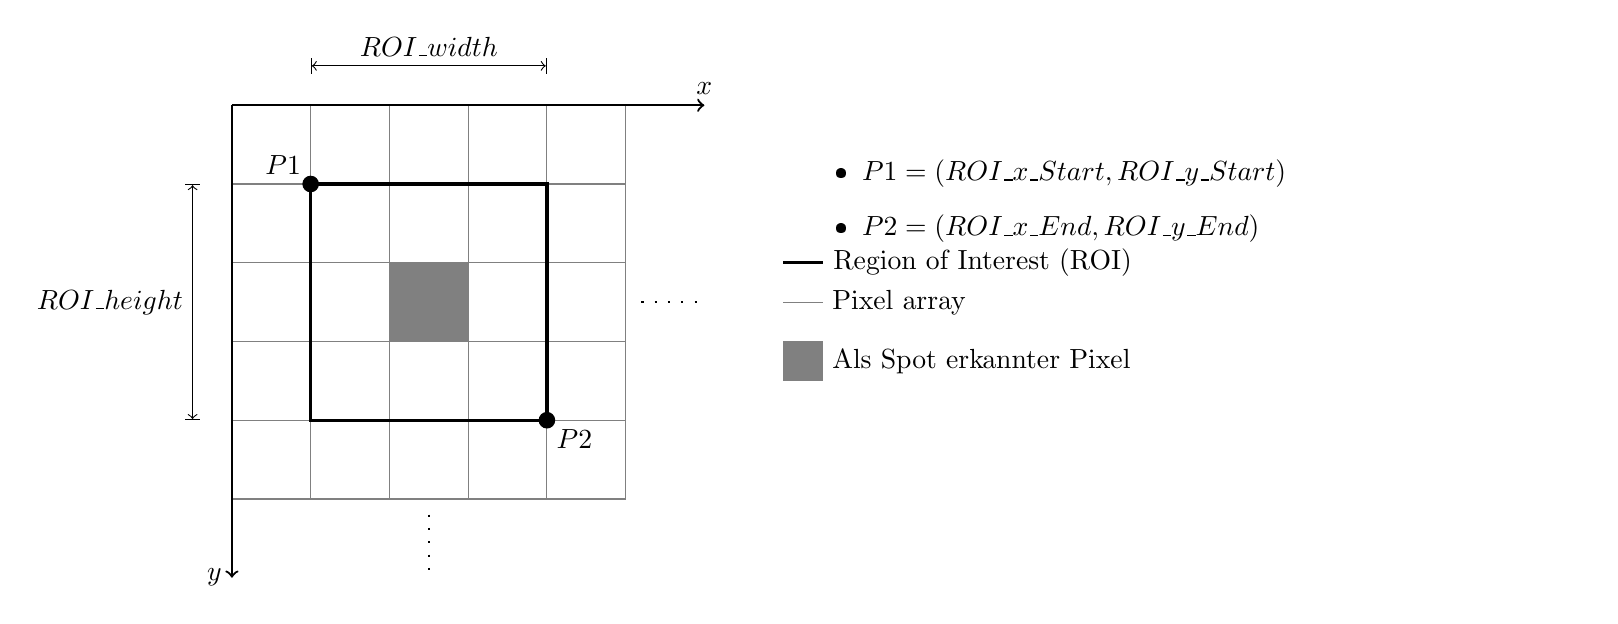
\begin{tikzpicture}
	\draw[gray]  (0,0) grid (5,5);
	\draw[very thick] (1,1) rectangle (4,4);
	\fill[gray] (2,2) rectangle (3,3);
	
	\draw[|<->|] (-0.5,1) -- node [left]{$ROI\_height$} (-0.5,4);
	\draw[|<->|] (1,5.5) -- node [above]{$ROI\_width$} (4,5.5);
	
	\fill (1,4) circle (3pt) node [above left]{$P1$};
	\fill (4,1) circle (3pt) node [below right]{$P2$};
	
	\draw[thick,->] (0,5)--(0,-1) node [left] {$y$};	
	\draw[thick,->] (0,5)--(6,5)node [above] {$x$};
	
	\draw[thick,loosely dotted] (2.5,-0.2)--(2.5,-1);
	\draw[thick,loosely dotted] (5.2,2.5)--(6,2.5);
	
	
	\node[right,text width=10cm] at (7,4) 
	{\begin{itemize}
		 \item $P1=(ROI\_x\_Start,ROI\_y\_Start)$
		 \item $P2=(ROI\_x\_End,ROI\_y\_End)$		
	\end{itemize}};
	
	\draw[very thick] (7,3)--(7.5,3) node [right]{Region of Interest (ROI)};
	\draw[gray] (7,2.5)--(7.5,2.5) node [right,black]{Pixel array};
	\fill[gray] (7,2) rectangle (7.5,1.5);
	\node[black] [right]at (7.5,1.75) {Als Spot erkannter Pixel};
	
	
\end{tikzpicture}

\textbf{Bildkorrektur der statischen Fehler:}

\begin{tikzpicture}[->,>=stealth']

	\node[initial,state,accepting,node distance=3cm]	(q0)	{$q_0$};
	\node[state,node distance=3cm]	(q1) [below left of=q0]  {$q_1$};
	\node[state,node distance=3cm]	(q2) [below right of=q0]  {$q_2$};
	
	\path[->]	(q0) edge [loop above] node[auto] {$\neg a$} (q0);
	\path[->]	(q0) edge [bend right] node[left] {$a \land b$} (q1);
	\path[->]	(q0) edge [bend left] node[right] {$a \land \neg b$} (q2);
	
	\path[->]	(q1) edge [loop left] node[auto] {$a$} (q1);
	\path[->]	(q1) edge [bend right] node[auto] {$\neg a$} (q0);
	
	\path[->]	(q2) edge [loop right] node[auto] {$a$} (q2);
	\path[->]	(q2) edge [bend left] node[right] {$\neg a$} (q0);

	\node[below right ,text width=10cm] at ($(q0)+(4, 1)$) 
	{\begin{itemize}
		\item \textbf{q\textsubscript{0}:} Warte-Zustand bis entweder die Initialisierung ausgelöst wird, oder ein Bild zur Korrektur zur Verfügung steht.
		\item \textbf{q\textsubscript{1}:} Initialisierungszustand, über ein Linux Programm wird ein Bild mit kurzer Belichtungszeit aufgenommen und in einen Block-RAM für die spätere Korrektur geschrieben.
		\item \textbf{q\textsubscript{2}:} Korrekturzustand, in dem nach der Initialisierung von den eingehendem Bild das Korrekturbild subtrahiert wird.
		\item
		\item \textbf{a:} write\_enable = true
		\item \textbf{b:} Init =true
	\end{itemize}};
	
\end{tikzpicture}

\textbf{Beschreibung Image Corrector:}\\
Der image\_corrector befindet sich zunächst in einem Wartezustand. Steht im main\_frame\_buffer ein Bild zur Verarbeitung bereit wird das Signal \textit{we} (write enable) auf 1 gesetzt. Das von einem Linux-Programm, über einen GPIO angesteuerte Signal \textit{init} bestimmt welche Funktionalität ausgeführt wird. Steht das Signal auf 1 wird das anliegende Bild in einen separaten Block-RAM geschrieben, bei einer 0 wird von dem anliegenden Bild, das Korrekturbild im Block-RAM subtrahiert und weitergegeben. Die Verarbeitung geschieht jeweils in Paketen von 32 Pixeln, mit je einem 8 Bit Helligkeitswert.